\documentclass[numerate]{cheatsheet}
\usepackage{bm}
\usepackage{textcomp, mathcomp}
\usepackage{empheq}
\usepackage{pbox}
\usepackage{booktabs}
\usepackage{cancel}
\usepackage{amssymb}
\usepackage{amsmath}

\newcommand{\doubleabs}[1]{\left\| #1 \right\|}


\doctitle{Control Systems 2 Cheatsheet}
\author{Noa Sendlhofer - nsendlhofer@ethz.ch}

\begin{document}
\section{Discrete Time}
	\subsection{Sampling}
    \begin{minipage}{0.49\linewidth}
        \centering \vspace{4pt}
        $T_s$: Sampling Time\\
        \vspace{2pt}
        $\omega_s$: Sampling frequency\\      
    \end{minipage}
    \begin{minipage}{0.49\linewidth}
        \centering
        $$
            \omega_s = \frac{2\pi}{T_s}
        $$
    \end{minipage}
	\subsection{Aliasing}
    \begin{align*}
        y_1[k] &= cos(\omega k T_s), &&k = 0, 1, 2\\
        y_2[k] &= cos((\omega + n\frac{2\pi}{T_s})k T_s), &&n = 0, 1, 2\\
        &= cos(\omega k T_s + \text{\cancel{$n2\pi k$}}) = y_1[k]
    \end{align*}
    \centerline{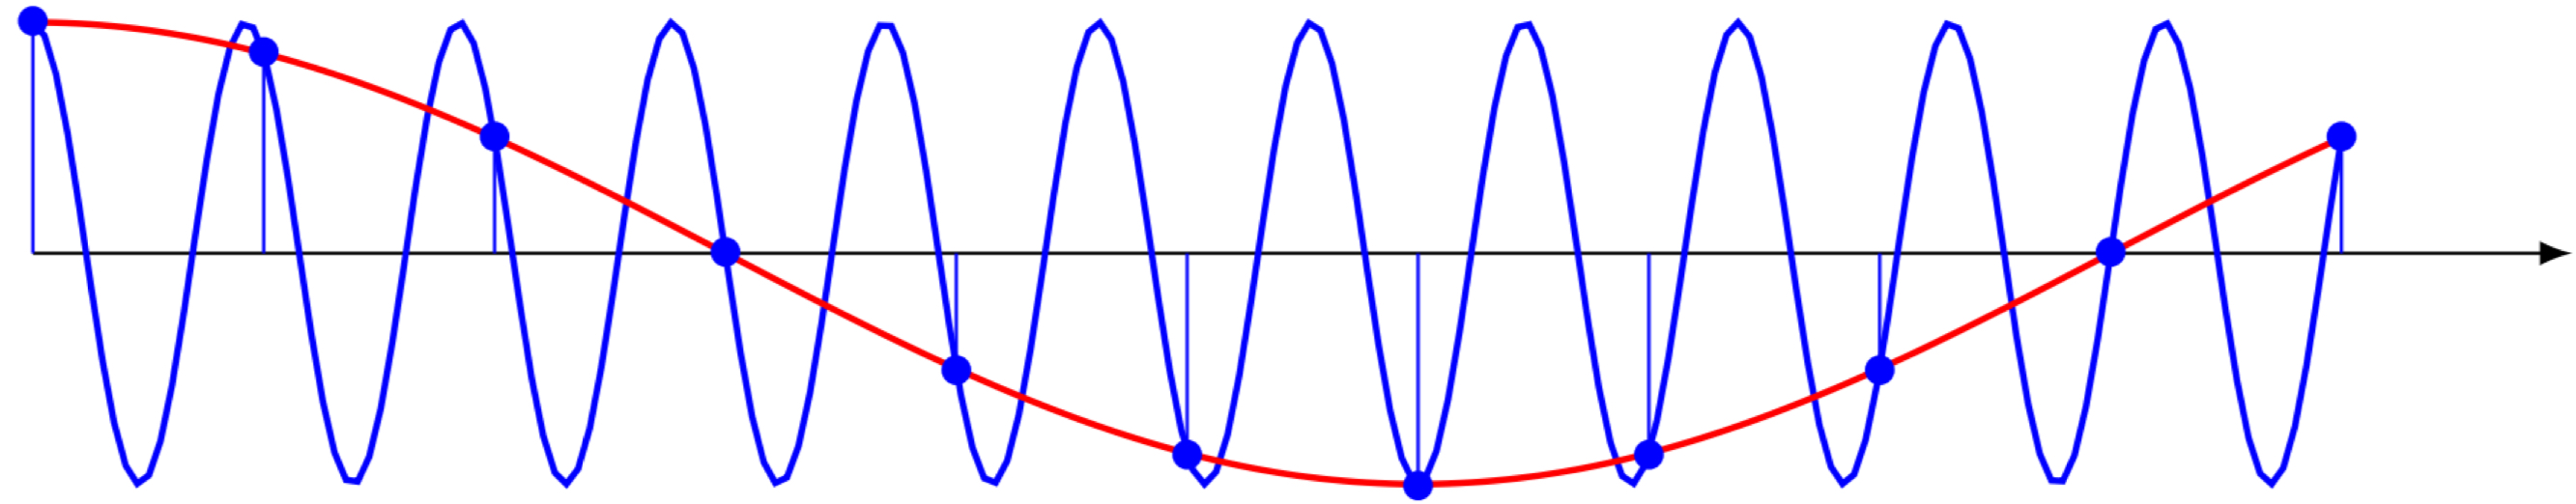
\includegraphics[width=0.8\linewidth]{src/1_discrete_time/images/aliasing.jpg}}
    \vspace{0pt}

    \subsubsection{Nyquist-Shannon Sampling theorem}
        $$
        f_N = \frac{1}{2T_s}\left[\text{Hz}\right] \quad \text{or} \quad \omega_N = \frac{\pi}{T_s}\left[\frac{\text{rad}}{\text{s}}\right]
        $$

        \centerline{\textbf{No aliasing if $\omega < \omega_N$!}}
	\subsection{DT State Space Representation}
    \begin{align*}
        x[k+1] &= A_d x[k] + B_d u[k]\\
        &= e^{A T_s} x[k] + \left(\int_{0}^{T_s} e^{A \tau}d\tau\right)B u[k]\\
        y[k] &= C_d x[k] + D_d u[k]\\
        &= C x[k] + D u[k]
    \end{align*}

    \quad If A is invertible: $B_d = A^{-1}(A_d - I)B$

    \subsubsection{Emulation}
        \centerline{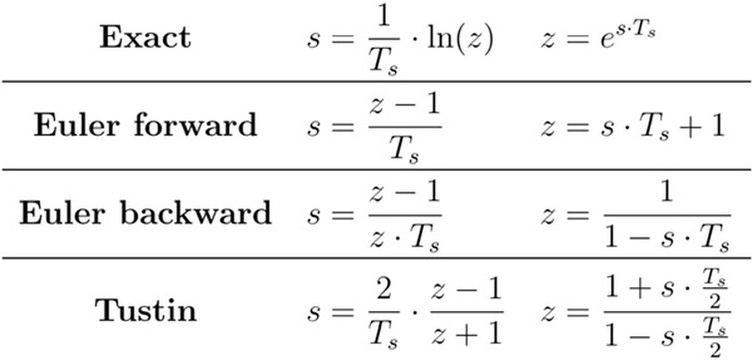
\includegraphics[width=0.8\linewidth]{src/1_discrete_time/images/emulation.jpeg}}
\section{System Properties}
	\subsection{Similarity Transformation}
    \begin{minipage}{0.43\linewidth}
        \vspace{1pt}
        \begin{equation*}
            \left\{
                \begin{aligned}
                    x^+ &= Ax + Bu\\
                    y &= Cx + Du
                \end{aligned}
            \right. \parbox[t]{0.7cm}{$\quad\Longrightarrow$}
        \end{equation*} 
    \end{minipage}
    \begin{minipage}{0.56\linewidth}
        \begin{equation*}
            \left\{
                \begin{aligned}
                    \tilde{x}^+ &= (T^{-1}AT)\tilde{x} + (T^{-1}B)u\\
                    y &= (CT)\tilde{x} + Du
                \end{aligned}
            \right.
        \end{equation*}
    \end{minipage}
    \vspace{2pt}

\subsubsection{Modal decomposition}
\vspace{-5pt}
\begin{minipage}{0.49\linewidth}
    \begin{equation*}
        \tilde{x}_i(t) = e^{\lambda_it}\tilde{x}_i(0)
    \end{equation*} 
\end{minipage}
\begin{minipage}{0.49\linewidth}
    \begin{equation*}
        x(t) = \sum_{i=1}^{n}e^{\lambda_it}\tilde{x}_i(0)v_i
    \end{equation*}
\end{minipage}
\vspace*{0.2em}
	\subsection{Reachability}
    \begin{minipage}{0.63\linewidth}
        $$
            \mathbf{R} := \left[A^{n-1}B | ... | AB | B \right] \in \mathbb{R}^{n\times n \cdot m}
        $$
    \end{minipage}
    \begin{minipage}{0.36\linewidth}
        $$
            \mathbf{U} :=
            \begin{bmatrix}
                u[0] \\
                u[1] \\
                \vdots \\
                u[n -1]
            \end{bmatrix}
        $$
    \end{minipage}

    $\Rightarrow x[n] = RU$
    \vspace{5pt}

    \textbf{The systen is reachable if and only if $\mathbf{R}$ has full row rank n}
	\subsection{Observability}
    \begin{minipage}{0.33\linewidth}
        \centering
        $\mathbf{O} = \begin{bmatrix} \strut C \\ \strut CA \\ \raisebox{0.5ex}{\vdots} \\  \strut CA^{n-1} \end{bmatrix}$
    \end{minipage}
    \begin{minipage}{0.32\linewidth}
        \centering
        $\mathbf{Y} = \begin{bmatrix} \strut y[0] \\ \strut y[1] \\ \raisebox{0.5ex}{\vdots} \\ \strut y[n-1] \end{bmatrix}$
    \end{minipage}
    \begin{minipage}{0.32\linewidth}
        \centering
        $\mathbf{Y} = \mathbf{O}x[0]$
    \end{minipage}
    \vspace{3pt}

    \textbf{The systen is observable if and only if $\mathbf{O}$ has full column rank n}
	\subsection{Controllability}
    A system is controllable if, for any initial condition $x_0$, there exists a control input $u$ that brings the state $x$ to $0$ in finite time.

    For CT Systems: Controllability = Reachability

    For DT Systems: A is invertible $\Rightarrow$ Controllability = Reachability
	\subsection{Kalman Decomposition}
\begin{align*}
    x^+ &= \begin{bmatrix}
        \Lambda_{r\overline{o}} & 0 & 0 & 0 \\
        0 & \Lambda_{ro} & 0 & 0 \\
        0 & 0 & \Lambda_{\overline{r}\overline{o}} & 0 \\
        0 & 0 & 0 & \Lambda_{\overline{r}o}
    \end{bmatrix} x + 
    \begin{bmatrix}
        B_{r\overline{o}} \\
        B_{ro} \\
        0 \\
        0
    \end{bmatrix} u, \\
    y &= \begin{bmatrix}
        0 & C_{ro} & 0 & C_{\overline{r}o}
    \end{bmatrix} x + Du
\end{align*}

\begin{itemize}
    \item \textbf{Stabilizability}\\
        A system is said to be stabilizable if all unstable modes are reachable

    \item \textbf{Detectability}\\
        A system is said to be detectable if all unstable modes are observable
\end{itemize}
\section{State Feedback}
	\subsection{State Feedback}
\centerline{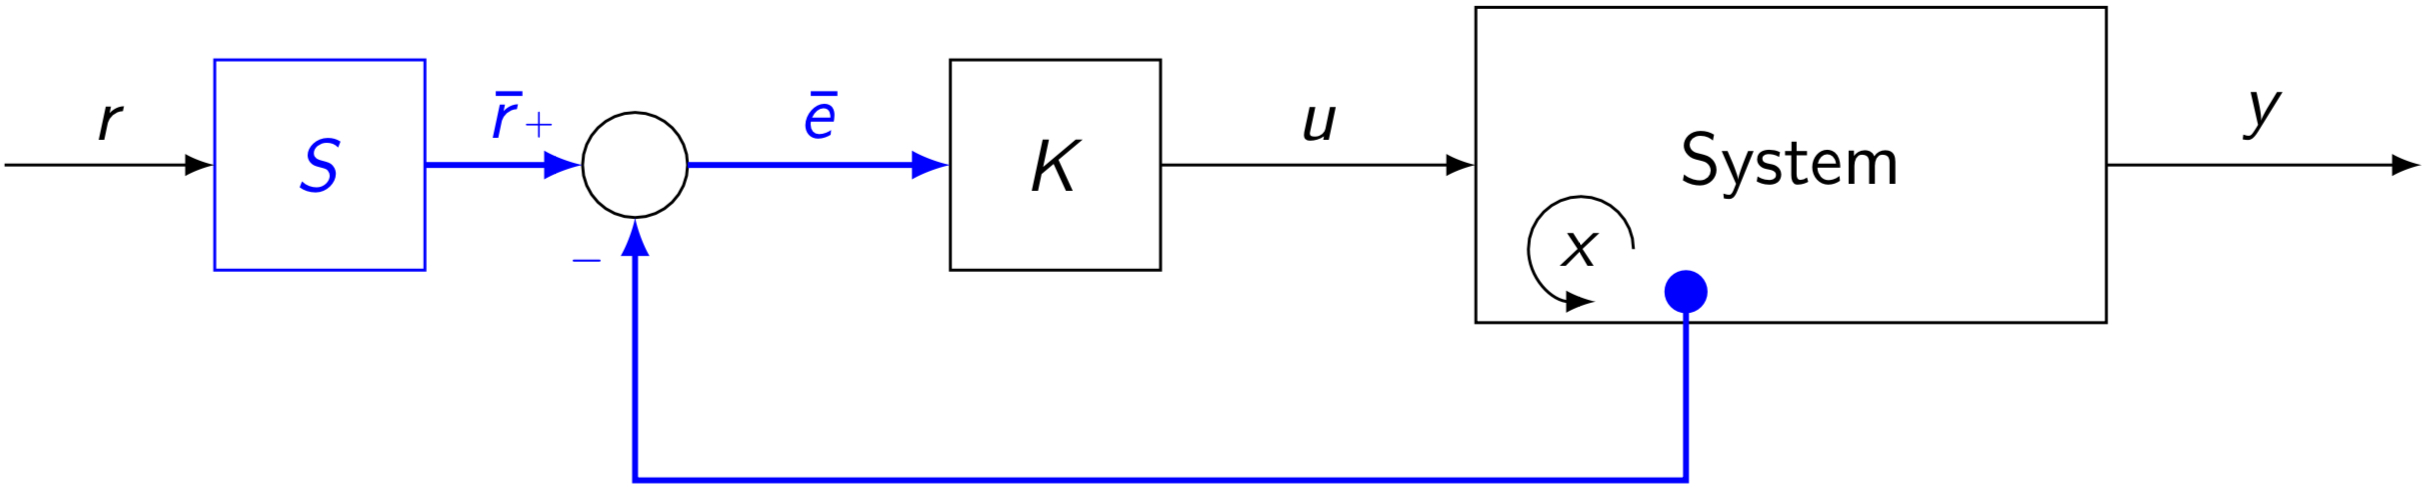
\includegraphics[width=0.95\linewidth]{src/3_state_feedback/images/state_feedback.jpeg}}
\begin{align*}
    \dot{x} &= (A-BK)x + BKSr\\
    &= (A-BK)x + B\overline{N}r, \qquad \overline{N} = KS\\
    y &= Cx + (D=0)\\[5pt]
    G_{yr}^{cl}(s) &= C(sI - A + BK)^{-1}BKS\\
    &= C(sI - A - BK)^{-1}B\overline{N}
\end{align*}

\subsubsection{$K$ - Direct Method}
$$
    p_{cl}^* = \prod_{i=1}^{n}(s + \lambda_i), \quad K = \begin{bmatrix} k_1 & k_2 & \hdots & k_n \end{bmatrix}
$$
$$
    p_{cl} = det(sI - A + BK) = p_{cl}^*
$$

\subsubsection{$K$ - Ackermann's Formula}
$$
    K = \begin{bmatrix} 0 & \hdots & 0 & 1 \end{bmatrix} \mathcal{R}^{-1}p_{cl}^*(A)
$$
\vspace*{0.1em}

\subsubsection{$S$}
$$
    \text{No steady-state error:} \Rightarrow G_{yr}^{cl}(0) = 1
$$
$$
    \Longrightarrow \overline{N} = - (C(A-BK)^{-1}B)^{-1}, \quad S = K^{-1}\overline{N}
$$
\vspace*{0.1em}
	\subsection{LQR}
LQR guarantees:
\begin{itemize}
    \item phase margin $\geq 60^\circ$
    \item gain margin ($\frac{1}{2}, +\infty$)
\end{itemize}

\subsubsection{Continuous Time}
    \vspace*{-0.4em}
    \begin{align*}
        \underset{K}{\text{min}} \, J(x,u) &= \int_{0}^{+\infty}[x(t)^TQx(t) + u(t)^TRu(t)]dt,\\[5pt]
        \text{s.t.:} \quad \dot{x}(t) &= Ax(t) + Bu(t),\\
        u(t) &= -Kx(t)\\[5pt]
        \text{soln.:} \qquad 0 &= A^TX + XA + Q - XBR^{-1}B^TX\\
        K &= R^{-1}B^TX
    \end{align*}

\subsubsection{Discrete Time}
    \vspace*{-0.4em}
    \begin{align*}
        \underset{K}{\text{min}} \, J(x,u) &= \sum_{k=0}^{+\infty}(x[k]^TQx[k] + u[k]^TRu[k]),\\[5pt]
        \text{s.t.:} \quad x[k+1] &= Ax[k] + Bu[k],\\
        u[k] &= -Kx[k]\\[5pt]
        \text{soln.:} \qquad X &= A^TXA - (A^TXB)(B'XB+R)^{-1}(B^TXA)\\
        &+Q\\
        K &= (R+B^TXB)^{-1}B^TXA
    \end{align*}

\subsubsection{LQR Servo}
    $$
    \begin{bmatrix} x \\ \epsilon \end{bmatrix} ^+
    = \begin{bmatrix} A & 0 \\ -C & 0 \end{bmatrix} \begin{bmatrix} x \\ \epsilon \end{bmatrix}
    + \begin{bmatrix} B \\ 0 \end{bmatrix} u + \begin{bmatrix} 0 \\ I \end{bmatrix} r
    $$
\end{document}